%%%%%%%%%%%%%%%%%%%%%%%%%%%%%%%%%%%%%%%%%%%
%%%%%%  STYLE 15
%%%%%%%%%%%%%%%%%%%%%%%%%%%%%%%%%%%%%%%%%%%
\newgeometry{left=2cm,right=7cm, marginparsep=15pt, marginparwidth=4.2cm,top=2cm}
\cxset{
 name={},
 numbering=none,
 number font-size=\LARGE,
 number font-family=\rmfamily,
 number font-weight=\bfseries,
 number before=,
 number dot=,
 number after=,
 number position=rightname,
 chapter font-family=\sffamily,
 chapter font-weight=\normalfont,
 chapter font-size=\Large,
 chapter before={},
 chapter after={},
 chapter color={black!90},
 number color=\color{purple},
 title beforeskip={},
 title afterskip={\vspace*{50pt}\par},
 title before={},
 title after={},
 title font-family=\rmfamily,
 title font-color=\color{black!80},
 title font-weight=\normalfont,
 title font-size=\Huge,
 title font-shape=\itshape,
 chapter opening=any,
 watermark text=SAMPLE PAGE,
 header style=samplepage}


\chapter{Introduction to Style Fifteen}

\parindent1em
\def\thefigure{\arabic{chapter}.\arabic{figure}}
\lorem\par

\marginpar{%
 {\centering
 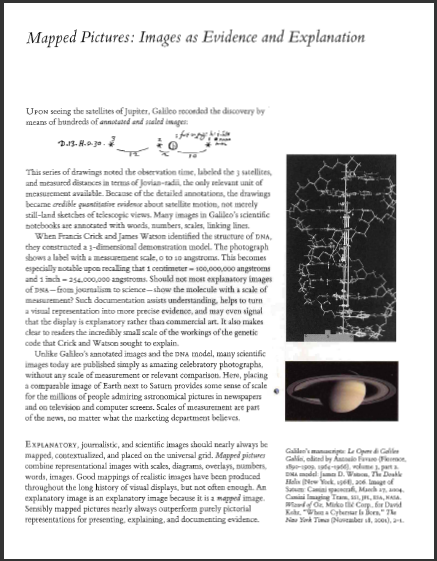
\includegraphics[width=4.2cm]{./chapters/chapter15}\vskip5pt\par}
 {\footnotesize\lorem}
}
\marginpar{%
{\centering
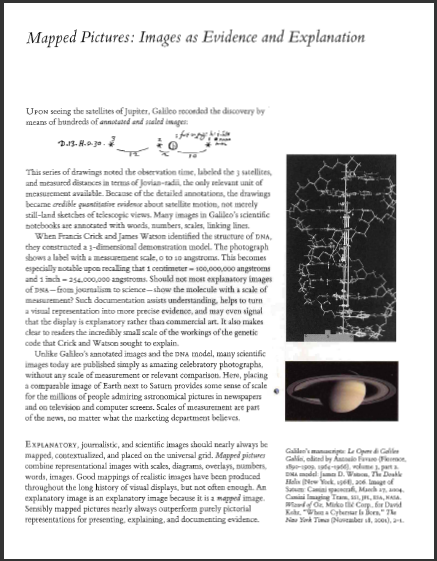
\includegraphics[width=4.2cm]{./chapters/chapter15}\par}
 { \captionof{figure}{\footnotesize\lorem}}
}
This is another marginpar of the same size.

\lorem

\lipsum
\marginpar{%
{\centering
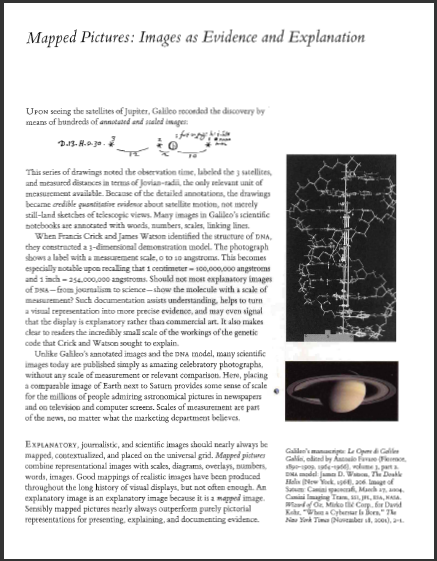
\includegraphics[width=4.2cm]{./chapters/chapter15}\par}
 { \captionof{figure}{\footnotesize\lorem}}
}
%%%% END STYLE %%%%%%%%%%%%%%%%%%%%%%%%%%%%%%%%%
